% Where the Task 3 error actually sits, by field strength.
% Compile from inside reports/:  ~/anaconda3/envs/tex/bin/tectonic error_by_field.tex
\documentclass[10pt,a4paper]{article}

\usepackage[margin=18mm]{geometry}
\usepackage{tikz}
\usepackage{booktabs}
\usepackage{xcolor}
\usepackage{amsmath}
\usetikzlibrary{arrows.meta}

\definecolor{src}{HTML}{2C6E8F}
\definecolor{tgt}{HTML}{C97B3C}
\definecolor{hot}{HTML}{C0392B}
\definecolor{muted}{HTML}{627D98}
\definecolor{rule}{HTML}{D9E2EC}

\pagestyle{empty}
\setlength{\parindent}{0pt}

% #1 y, #2 label, #3 source share, #4 target share, #5 bar opacity
\newcommand{\bars}[5]{%
  \node[font=\small, anchor=east] at (-0.25,#1) {#2};
  \fill[src, opacity=#5] (0,#1+0.13) rectangle (#3*0.285,#1+0.40);
  \fill[tgt, opacity=#5] (0,#1-0.40) rectangle (#4*0.285,#1-0.13);
  \node[font=\scriptsize, text=src, anchor=west] at (#3*0.285+0.1,#1+0.265) {#3\%};
  \node[font=\scriptsize, text=tgt, anchor=west] at (#4*0.285+0.1,#1-0.265) {#4\%};}

\begin{document}

{\Large\bfseries Where the error is}\\[1mm]
{\small Task 3, model \texttt{mc+ssim e8} (challenge SSIM 0.908873). 180 transitions ---
3 paired subjects $\times$ 3 modalities $\times$ 20 ordered field pairs, scored locally.
Error is $1-\mathrm{SSIM}$ summed over transitions; total $=7.7248$.}\\[4mm]

\begin{minipage}[t]{0.46\textwidth}
\vspace{0pt}
\small
\begin{tabular}{lrrrr}
\toprule
& \multicolumn{2}{c}{as \textcolor{src}{source}} & \multicolumn{2}{c}{as \textcolor{tgt}{target}} \\
\cmidrule(lr){2-3}\cmidrule(lr){4-5}
Field & SSIM & err.\ & SSIM & err.\ \\
\midrule
\textbf{0.1\,T} & \textbf{0.9432} & \textbf{26.5\%} & \textbf{0.9495} & \textbf{23.6\%} \\
1.5\,T          & 0.9582 & 19.5\% & 0.9542 & 21.3\% \\
3\,T            & 0.9656 & 16.0\% & 0.9550 & 21.0\% \\
5\,T            & 0.9630 & 17.2\% & 0.9592 & 19.0\% \\
7\,T            & 0.9554 & 20.8\% & \textbf{0.9676} & \textbf{15.1\%} \\
\midrule
total           &        & 100\%  &        & 100\% \\
\bottomrule
\end{tabular}

\vspace{2mm}
{\footnotesize Each column sums to 100\%: every transition has exactly one source and one
target, so the two decompositions are separate partitions of the same total error.}
\end{minipage}\hfill
\begin{minipage}[t]{0.5\textwidth}
\vspace{0pt}
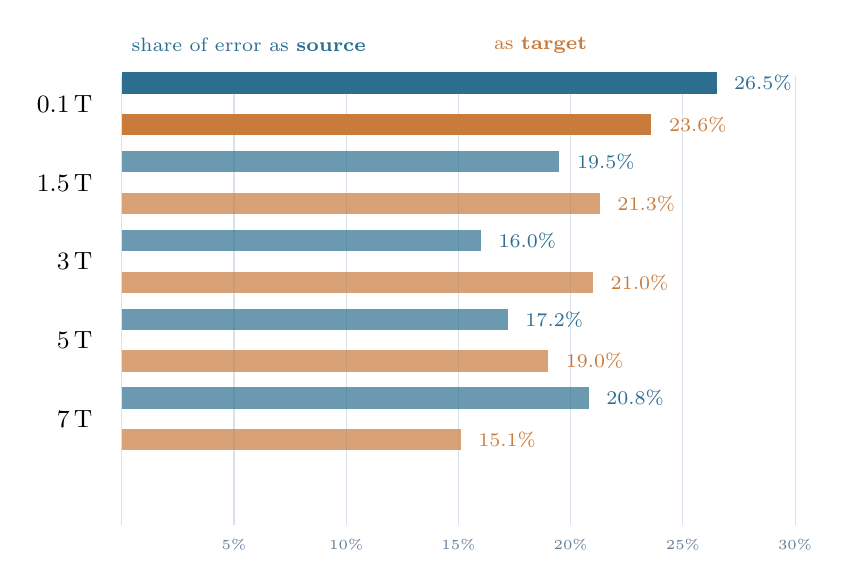
\begin{tikzpicture}[x=1cm,y=1cm]
  \draw[rule] (0,-0.35) -- (0,5.35);
  \foreach \x in {5,10,15,20,25,30}{
    \draw[rule] (\x*0.285,-0.35) -- (\x*0.285,5.35);
    \node[font=\tiny, text=muted] at (\x*0.285,-0.6) {\x\%};}
  \bars{5.0}{0.1\,T}{26.5}{23.6}{1.0}
  \bars{4.0}{1.5\,T}{19.5}{21.3}{0.7}
  \bars{3.0}{3\,T}{16.0}{21.0}{0.7}
  \bars{2.0}{5\,T}{17.2}{19.0}{0.7}
  \bars{1.0}{7\,T}{20.8}{15.1}{0.7}
  \node[font=\scriptsize, text=src, anchor=west] at (0,5.75) {share of error as \textbf{source}};
  \node[font=\scriptsize, text=tgt, anchor=west] at (4.6,5.75) {as \textbf{target}};
\end{tikzpicture}
\end{minipage}

\vspace{5mm}
{\small
\textbf{0.1\,T is 40\% of the transitions and exactly 50\% of the error.} The 72 transitions with
0.1\,T at either end carry half the total, against the 40\% they would carry if error were spread
evenly. It is the worst field in both roles --- hardest to map \emph{from} (0.9432, the lowest
number in the table) and second hardest to map \emph{to}.

\textbf{The asymmetry is informative.} 7\,T is the \emph{easiest} target (0.9676) and among the
harder sources (0.9554); 3\,T is the easiest source (0.9656) but a middling target. Mapping
toward high field is easier than mapping away from it, which is what one expects if the models
are effectively learning to add plausible detail rather than to remove it: information can be
invented convincingly, but discarding it correctly requires knowing what the low-field
acquisition would actually have lost.

\textbf{What this is worth.} If transitions touching 0.1\,T merely scored what the rest do
(0.96426 against their 0.94632), the overall local score would move
$0.95708 \rightarrow 0.96426$, i.e.\ \textbf{+0.0072}, projecting to roughly \textbf{0.9126} on
the challenge against our 0.908873 and the current frontier's 0.916747. That single domain is
most of the remaining gap.

\textbf{Caveat on the obvious next step.} The natural reading is ``0.1\,T is the low-SNR regime,
so model its noise'' --- and two of the teams above us have \texttt{rician} and \texttt{noisy} in
their submission names. But a direct test on this data could not confirm a Rician model: the
background is masked to zero (no $\nu=0$ population to fit), and two independent estimators of
$\sigma$ versus signal level disagree in opposite directions, one confounded by anatomical
texture and the other by mask edges. Registration and resampling also average neighbouring
voxels, which pushes any marginal toward Gaussian. Better to measure the empirical conditional
$p(\text{0.1\,T} \mid \text{high field})$ from the three paired subjects, which we have, than to
assume a parametric noise family we cannot verify.}

\end{document}
